\chapter[Cronograma]{Cronograma}
\label{chap:crono}

A Figura \ref{img:cronograma} mostra o cronograma das atividades realizadas durante a primeira parte do projeto.

\begin{figure}[H]
    \centering
    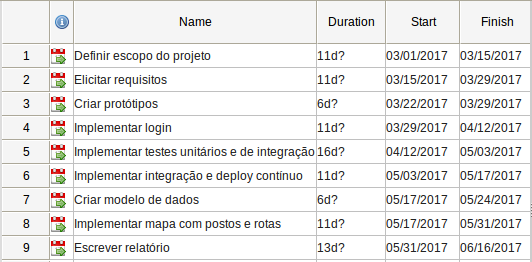
\includegraphics[scale=0.5]{figuras/cronograma_r1.png}
    \caption[Cronograma de atividades da primeira entrega.]{Cronograma de atividades da primeira entrega. Fonte: autores}
    \label{img:cronograma}
\end{figure}

Na Figura \ref{img:cronograma2inicial} temos o cronograma inicial da segunda parte do projeto.

\begin{figure}[H]
    \centering
    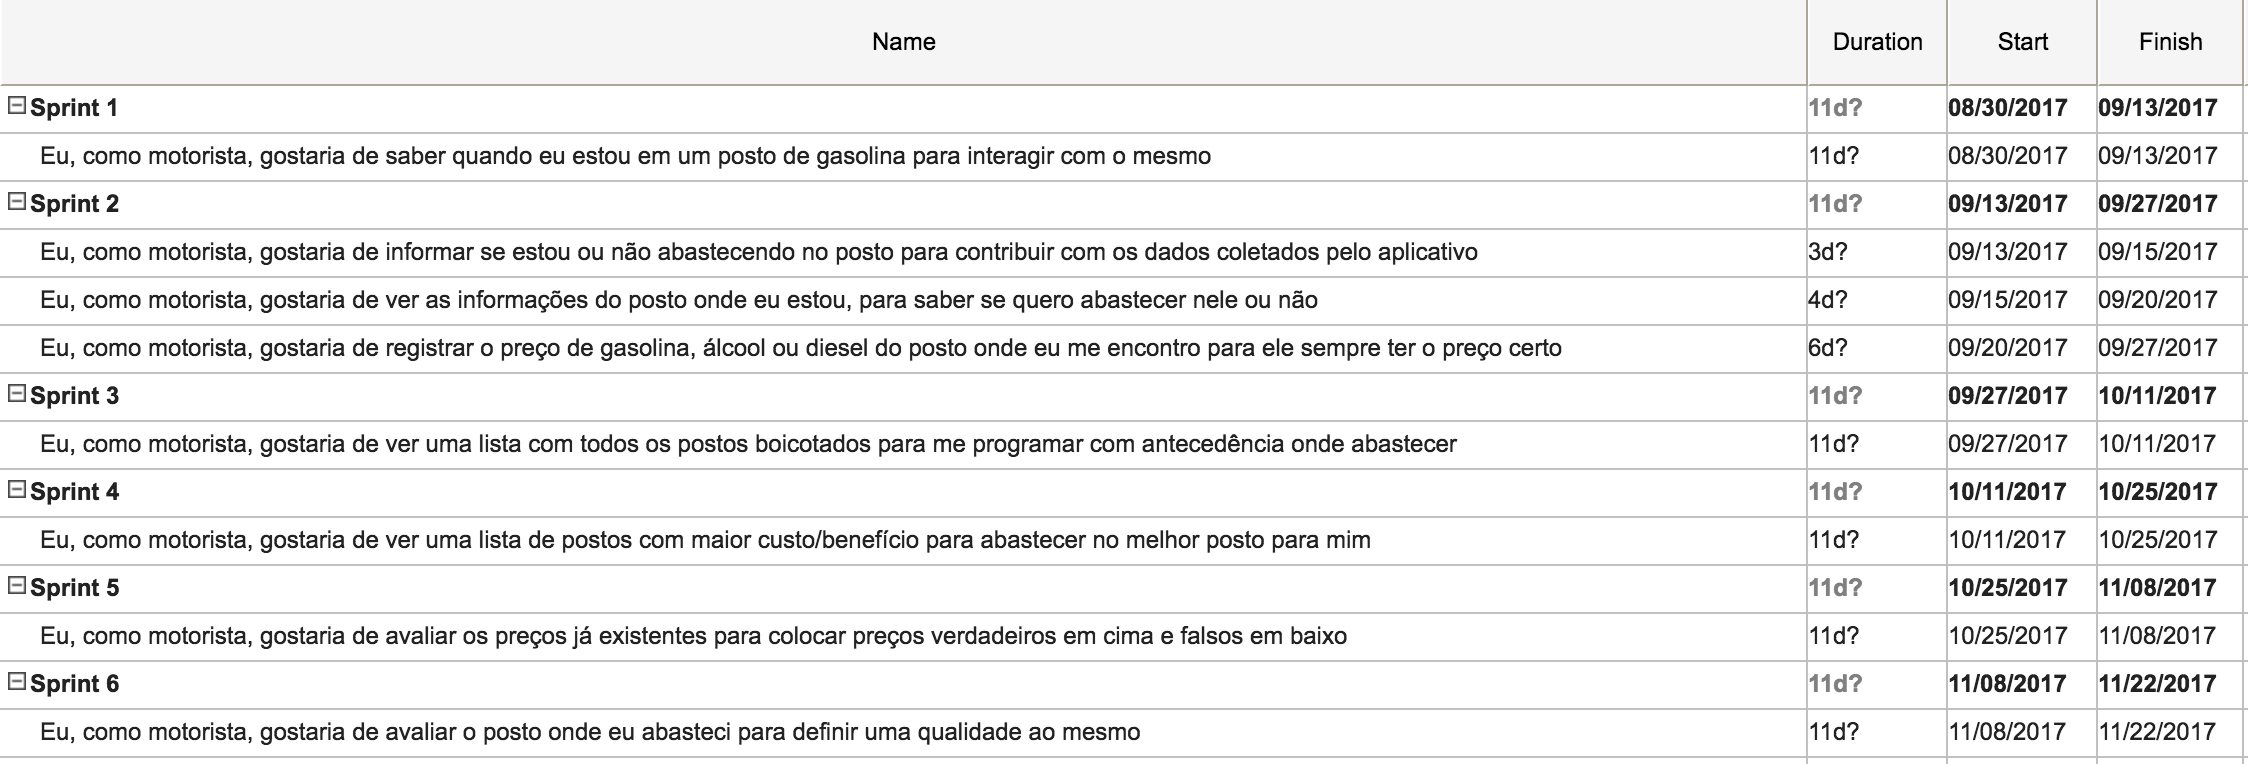
\includegraphics[scale=0.4]{figuras/cronograma_segunda_parte_1.png}
    \caption[Cronograma inicial de atividades da segunda entrega.]{Cronograma inicial de atividades da segunda entrega. Fonte: autores}
    \label{img:cronograma2inicial}
\end{figure}

Porém, devido a certas adversidades e melhor compreensão do projeto, foram feitas certas mudanças no cronograma como mostra a Figura \ref{img:cronogramafinal}.

\begin{figure}[H]
    \centering
    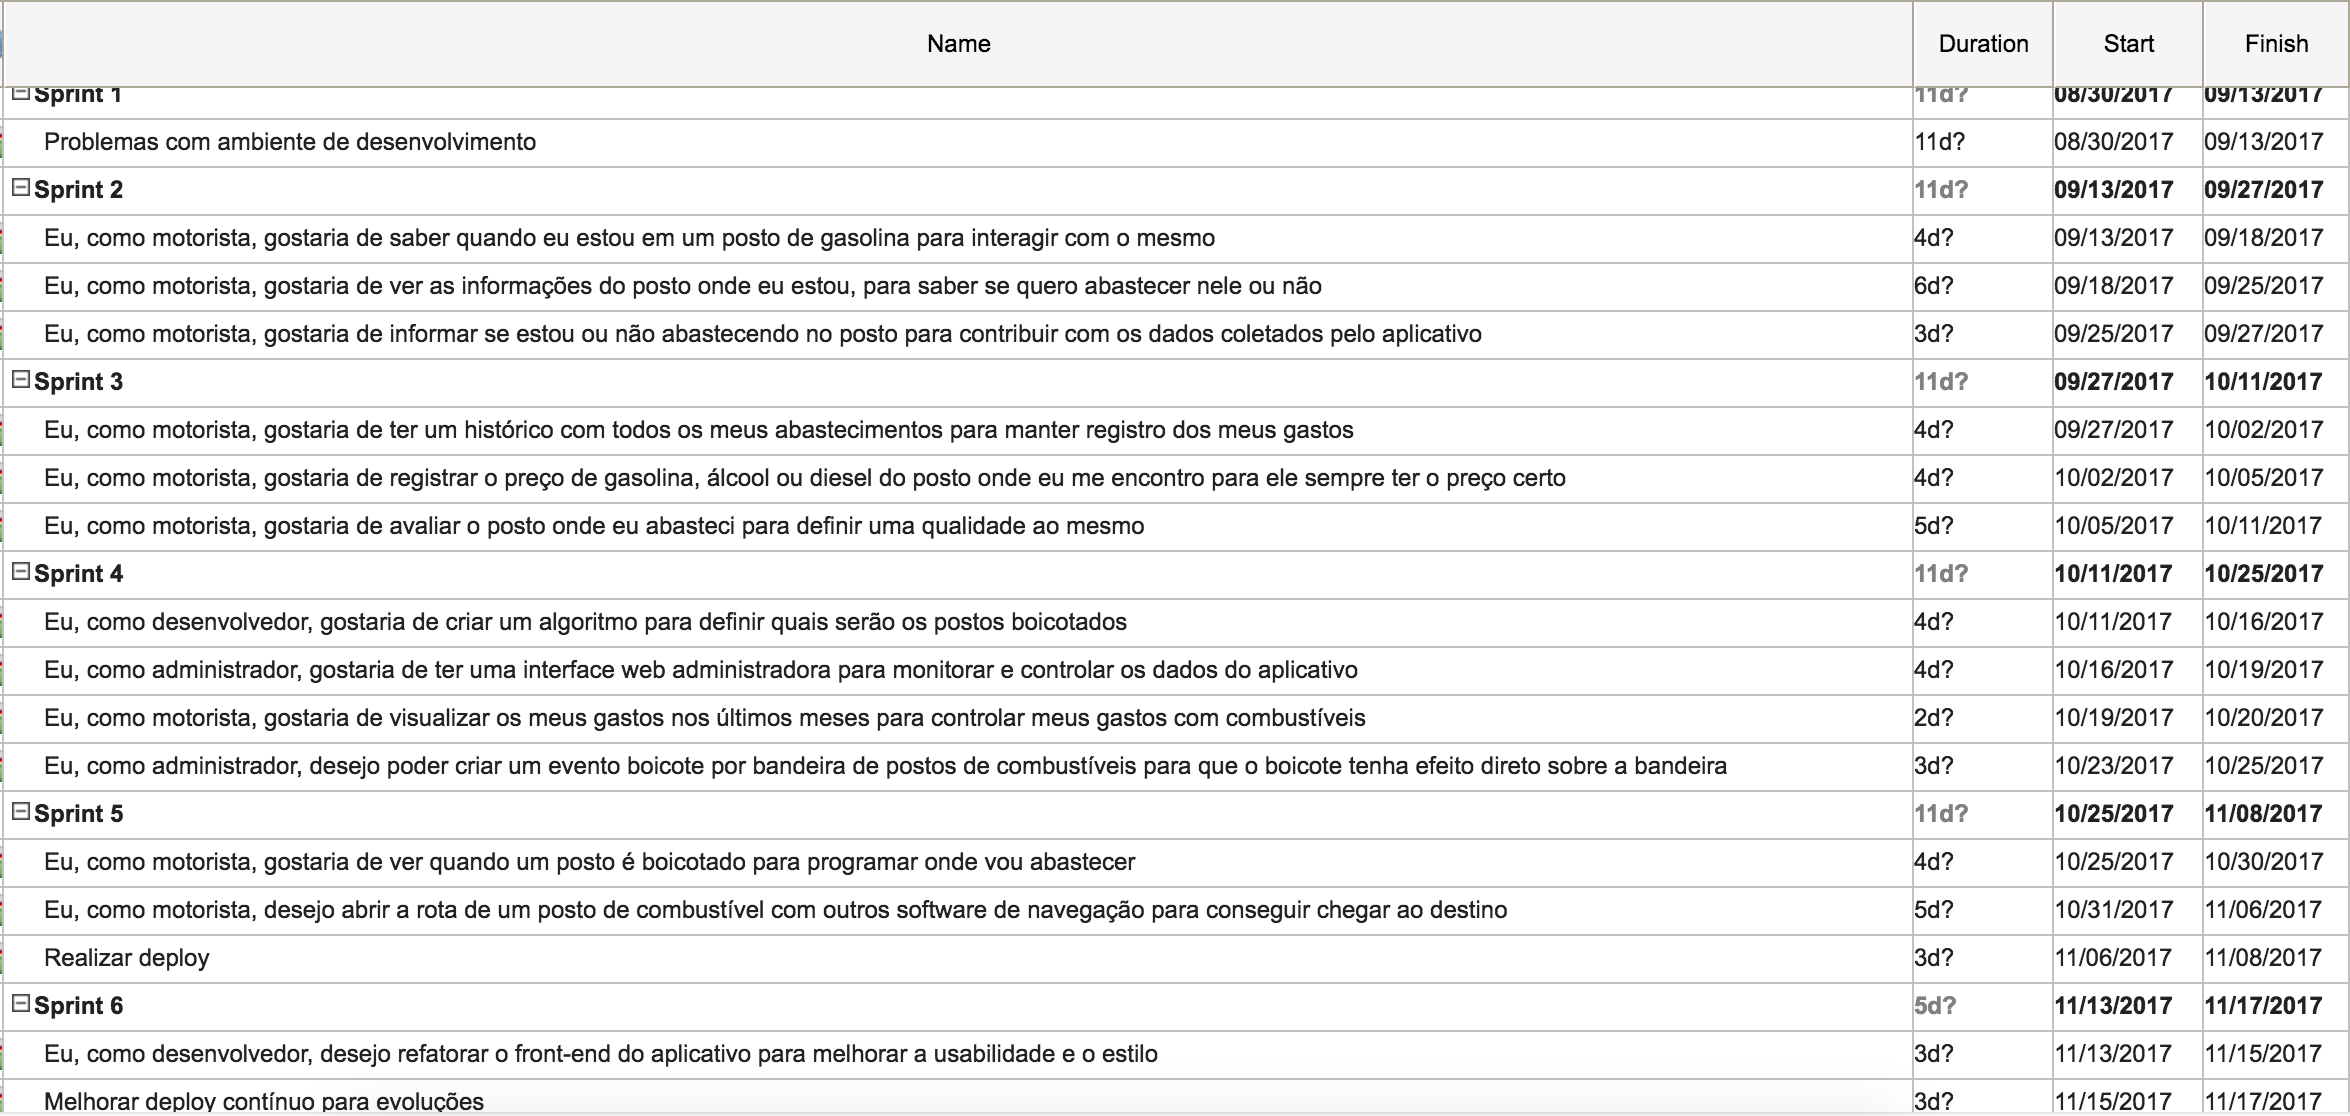
\includegraphics[scale=0.4]{figuras/cronograma_segunda_parte_2.png}
    \caption[Cronograma final de atividades da segunda entrega.]{Cronograma final de atividades da segunda entrega. Fonte: autores}
    \label{img:cronogramafinal}
\end{figure}

Principalmente na primeira sprint, tivemos muitos problemas com o Ionic por causa das atualizações do Ionic 2 para o Ionic 3.

EXPLICAR TRETA DO IOS.

Além do problema da plataforma da Apple, o \textit{plugin} do \textit{Geofences}, o plugin utilizado para definir cercas geográficas nos postos para indicar para o usuário quando ele entra em um posto de gasolina, não atualizou todas as funcionalidades corretamente, principalmente a funcionalidade de \textit{push notification}. Por causa desse problema, o projeto acabou atrasando mais do que devia pois foi necessário realizar mais pesquisas sobre novas alternativas. Por fim, foi utilizado o \textit{push notification} da Google utilizando o Firebase.

Durante a sprint 5, percebeu-se que seria necessário uma tela de administração para poder definir os ícones dos postos assim como corrigir quaisquer informações incorretas vindo das fontes externas e por isso foi adicionado no cronograma. Durante a mesma sprint, viu-se necessário melhorar a inteface do aplicativo pois o foco até então foi exclusivamente em desenvolver as funcionalidades. Porém, esse melhoria foi alocada para a sprint 6 por que a sprint 5 já possuia muitas tarefas.
